\section{Introduction}
In this chapter we build on the empirical heat maps in Chapter 1. First, we develop a statistical model for spatial variation in hitter success probabilities. This involves generalized linear models (GLMs), some biomechanics, and polar coordinates. Second, we focus on heat map confidence intervals. We take a look at current best practices, and then provide an alternative.

\section{A Generalized Linear Model for Hitter Success Probabilities} % =========================

\subsection{Preliminaries}

We aim to create a statistical model to explain the variation of success probabilities through the hitting zone. Nonparametric methods, lacking contextually interpretable parameters, limit interpretability. We propose a parametric approach using biomechanically interpretable covariates. Existing research analyzes the biomechanics of the baseball swing \citep{Welch1995}, but no research links those results to spatial hitting results in a statistical model. To begin, we define preliminary indices and notation.

Let success indicator variable $Y_{ijklm}$ define a Bernoulli random variable with spatially varying mean \citep{Ross2002}. Let subscript $i = 1, \dots, n_{jklm}$ index hitter $j$ swings, in at bat $k$, against pitcher $l$, in year $m$. Let subscript $k = 1, \dots, n_{jlm}$ index hitter $j$ at bats against pitcher $l$, in year $m$. Let subscript $l = 1, \dots, n_{jm}$ index pitchers that hitter $j$ faced, with hitter-pitcher total $n_{jm}$; and let $m = 2007, \dots, 2016$ index year. Let $\pmb{s}_{ijkl} = (px_{ikl}, pz_{ijkl})\in \pmb{D} \subseteq \pmb{R}^{2}$ define the horizontal and vertical locations, respectively, of pitch $ijkl$ as it passes through the two dimensioned vertical face of the hitting zone\footnote{PITCHf/x\textsuperscript{\textregistered} records pitch locations in a three-dimensional coordinate system with horizontal x-axis, vertical z-axis, and y-axis running from the pitchers mound through home plate.}. The origin, $\pmb{s} = (0,0)$, lies at midpoint of the front edge of home plate, at ground level. From the umpire's point of view, pitches to the left of the origin correspond to negative values of $px$. Pitches that bounce before reaching home plate correspond to negative values of $pz$.  

In this study we make the simplifying assumption that location success probabilities depend on location and hitter only. Therefore, we dispense with subscripts $k, l,$ and $m$. We also assume, in this chapter, that swings occur---given hitter $j$ and pitch location $\pmb{s}_{ij}$---as statistically independent Bernoulli trials. Therefore, $Y_{ij}|\pmb{s}_{ij} \sim \text{Bernoulli}(p_{ij})$ where $\text{E}[Y_{i}|\pmb{s}_{ij}] = p_{ij}$. Accordingly, we revise and simplify the notation: let $i = 1, \dots, n_{j}$ index hitter $j$ swings, out of $n_{j}$ total recorded swings; and let vector $\pmb{X}_{ij}(\pmb{s}_{i})$ denote hitter $j$, location $\pmb{s}_{ij}$, swing $i$ covariates. A Bernoulli random variable suggests logistic regression, a GLM with logit link function, for relating covariate information to spatial success probability \citep{Myers2012}. The logit link, $logit(p) = log\left[p/(1-p)\right]$, maps $p$ with support $(0,1)$ to the positive real numbers. A GLM with logit link constitues a logistic regression equation, given by: 

\begin{equation}
\text{logit}(p_{ij}|\pmb{X}_{ij}(\pmb{s}_{ij})) = \pmb{X}_{ij}(\pmb{s}_{ij}) \pmb{\beta}_{j}.
\end{equation}

Vector of covariate coefficients $\pmb{\beta}_{j}$ contains parameters specific to hitter $j$. Next, we discuss and develop covariates.

\subsection{Rotational Biomechanics} % ==============

Why does Jhonny Peralta, and hitters in general, hit pitches in some locations better than others? We propose biomechanics underpin hitter location preferences. Notice that athletes, given the choice, carefully position their ball before swinging. Consider golf, a sport with a stationary ball, where the athlete chooses the exact athlete-to-ball distance, depth, and angle. 
  \begin{figure}[H]
	\centering	
	\includegraphics[scale=.45]{Images/Golf.jpg}
  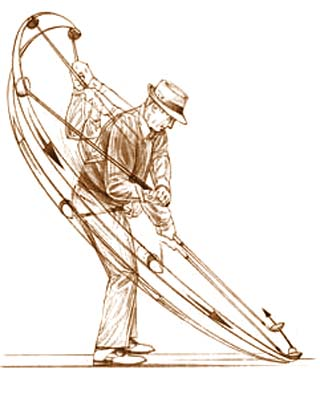
\includegraphics[scale=.6]{Images/Snead.jpg}
	\caption{Golfers position themselves with careful precision in relation to the ball, to achieve optimal impact. Deviations from this ideal lead to biomechanical adjustments and suboptimal results \citep{Cochran2005}.}
	\end{figure}
Indeed, golfers position themselves very precisely in relation to the ball to achieve optimal impact \citep{Cochran2005}. If the impact point deviates from the optimal location biomechanical adjustments hurt performance. Or consider tennis, similar to baseball in that a moving ball approaches, but different in that the player has freedom to position him/herself relative to the incoming ball. Once again, tennis players strive to hit the ball at a specific point in their stroke, a precise distance from the ground and from their body, with precise depth \citep{Elliott2006}. 
  \begin{figure}[H]
	\centering	
	\includegraphics[scale=.4]{Images/tennis2.jpeg}
	\caption{Tennis players strive to hit the incoming tennis ball at a precise height and distance from their torso. Deviations from this ideal height and distance lead to a series of biomechanical adjustments, and ultimately suboptimal results \citep{Elliott2006}.}
	\end{figure}
As with golf, if the point of impact deviates from from the optimal location, biomechanical adjustment ensue, and performance suffers. Tennis provides a strong example, because players have {\it some} control over the point of impact, and results demonstrate the consequence of varying points of impact. For example, even novice viewers observe that a player barely reaching a ball returns it, on average, with less velocity and precision than a ball he/her has time to set up for.  

In both golf and tennis the ideal player-to-ball positioning depends on, at the very least, anatomy, biomechanics, and equipment. We submit the same dynamics affect baseball hitting. However, in baseball the hitter reacts to unpredictable ball location, without time to reposition him/herself in response to the location and trajectory of the incoming pitch. For these reasons, we turn to hitter-to-ball distance and angle measurements for covariates. 

\section{Biomechanical Covariates}

Future research may incorporate physical characteristics specific to individual hitters. At this stage we focus on biomechanical information content captured in pitch locations. To produce biomechanical covariates, we convert (rectangular coordinate) pitch locations to polar coordinates with a translated origin. As illustrated in Figure 3.3, we shift the origin to the bat's approximate moment-of-intertia (MOI) for a league average 6'2" hitter \citep{Fleisig}. The MOI coincides approximately with the intersection of the bat line at the moment of contact and the hitter's axis of rotation \citep{Welch1995}.
  \begin{figure}[H]
	\centering
	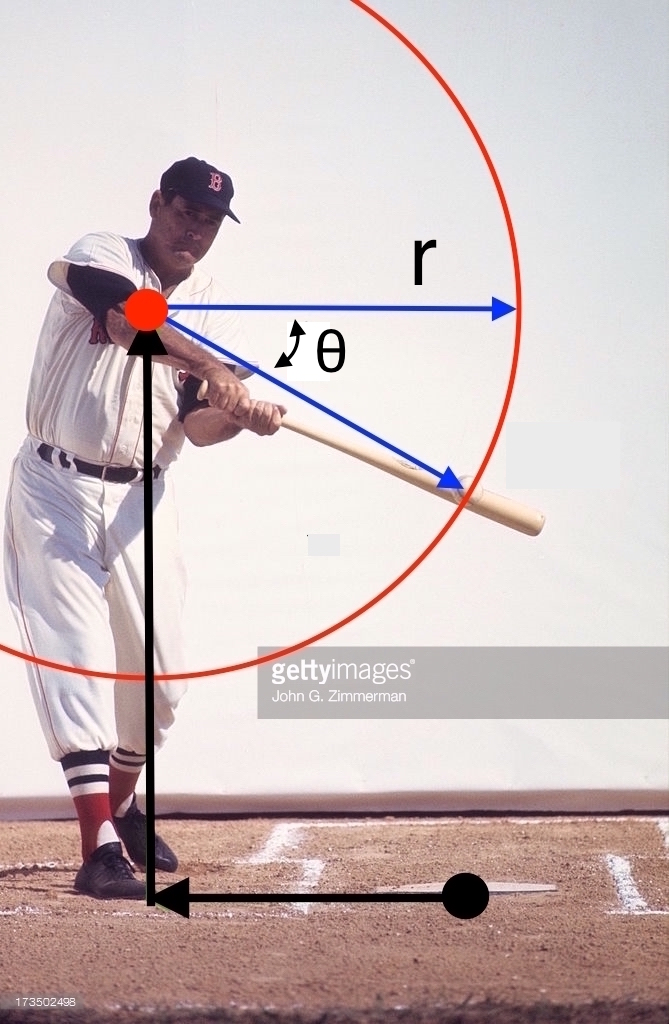
\includegraphics[scale=.16]{Images/WilliamsPolar.jpg}
	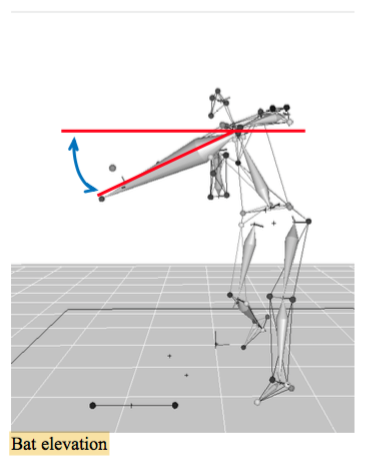
\includegraphics[scale=.07]{Images/Elevation.jpg}
	\caption{Ted Williams in ``The Science of Hitting,'' and baseball swing kinematic analysis at the American Sports Medical Institute \citep{Fortenbaugh2011}. We translate the origin (black dot) and rectangular coordinates to the new origin (red dot) in polar coordinates. We located the new origin at the bat's approximate moment of intertia (MOI) \citep{Fleisig}. Polar coordinates component $r$ gives the MOI-to-ball distance, and $\protect\theta$ gives the bat ``elevation.''}
	\end{figure}
Polar coordinate $r$ measures the distance, at contact, from the MOI to the ball. The kinematic analysis image on the right shows bat ``elevation,'' the angle below horizontal of the bat line, which serves as polar coordinate component $\theta$ \citep{Fortenbaugh2011}. 

As in golf and tennis, hitter-to-ball distances---too close to/far from the hitter, above/below the ideal point of impact---affect hitting performance. We use $r_{ij}$ and $\theta_{ij}$ terms for $\pmb{X}_{ij}(\pmb{s}_{ij})$ in equation 3.1.

\subsection{Generalized Linear Model} % =========================

Further biomechanical research extends beyond the scope of this study. Therefore, without biomechanical knowledge to inform us otherwise, we use $r$ and $\theta$ linear, quadratic, and interaction terms as covariates in our GLM linear predictor; $\pmb{X}_{ij}(\pmb{s}_{ij}) = \{r_{ij}, \theta_{ij}, r_{ij}\theta_{ij}, r_{ij}^{2}, \theta_{ij}^{2}, r_{ij}^{2}\theta_{ij}^{2}\}$. With $6 \times 1$ covariate vector $\pmb{X}_{ij}(\pmb{s}_{ij})$ in hand, we can define $\pmb{\beta}_{j}' =  \{\beta_{j0}, \beta_{j1}, \dots, \beta_{j6}\}$, and recall:

\begin{equation}
\text{logit}(p_{ij}|\pmb{X}_{ij}(\pmb{s}_{ij})) = \pmb{X}_{ij}(\pmb{s}_{ij}) \pmb{\beta}_{j}.
\end{equation}

% \begin{equation}
% \text{logit}(p_{ij}|\pmb{X}_{ij}(\pmb{s}_{ij})) = \beta_{j0} + \beta_{j1}r_{ij} + \beta_{j2} \theta_{ij} + \beta_{j3} r_{ij} \theta_{ij} +  \beta_{j4}r_{ij}^{2} + \beta_{j5} \theta_{ij}^{2} + \beta_{j6} r_{ij}^{2} \theta_{ij}^{2}
% \end{equation}

Note that given a hitter $j$, and pitch location $\pmb{s}_{ij}$, the elements of $\pmb{X}_{ij}$ are simply a trigonemtric function of $\pmb{s}_{ij}$ and the translated origin.

As a first step in exploring the effectiveness of the approach developed above, we fit the model to Johnny Peralta data (see Chapter 1). Let $j = P$, denoting player (P)eralta. We use Peralta's $n_{\text{P}} = 9177$ observed swings, and find maximum likelihood estimates of $\pmb{\beta}_{\text{P}}$ using an iteratively reweighted least squares algorithm \citep{Myers2012}. Figure 3.4 shows the Peralta empirical and fitted heat maps.
  \begin{figure}[!ht]
    \centering
    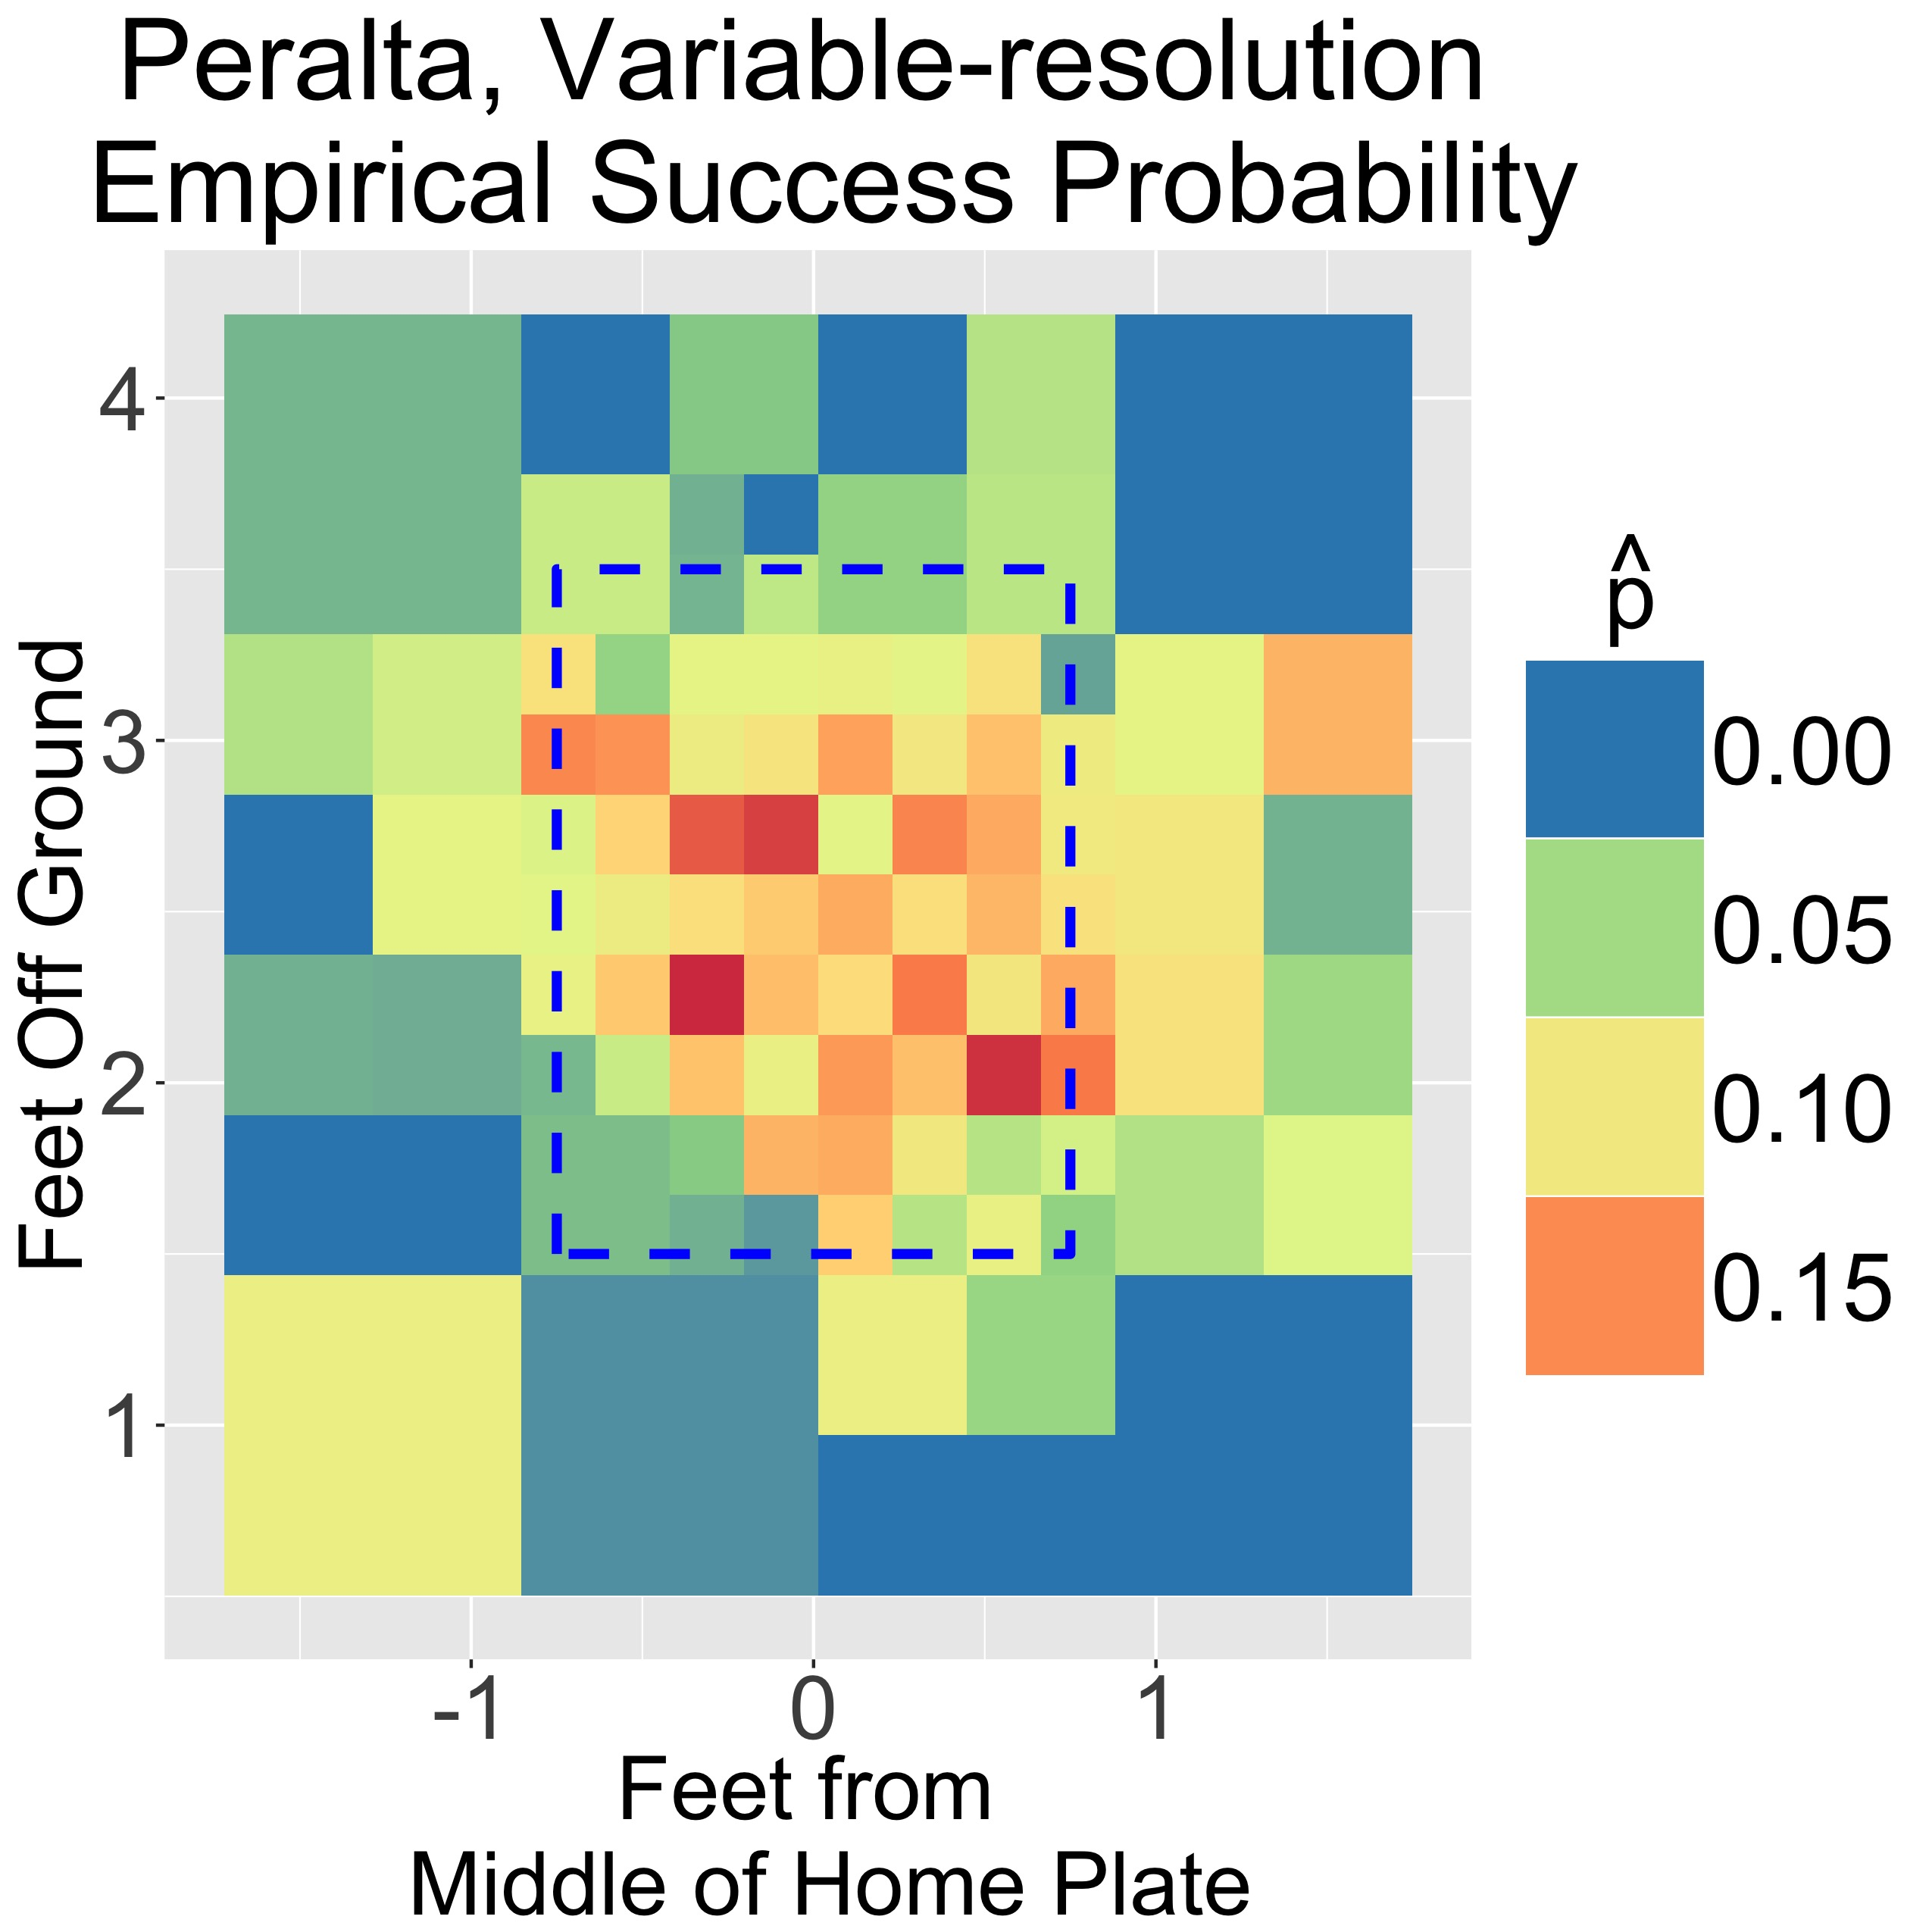
\includegraphics[scale=.08]{Images/Peralta_var-res.jpg}
    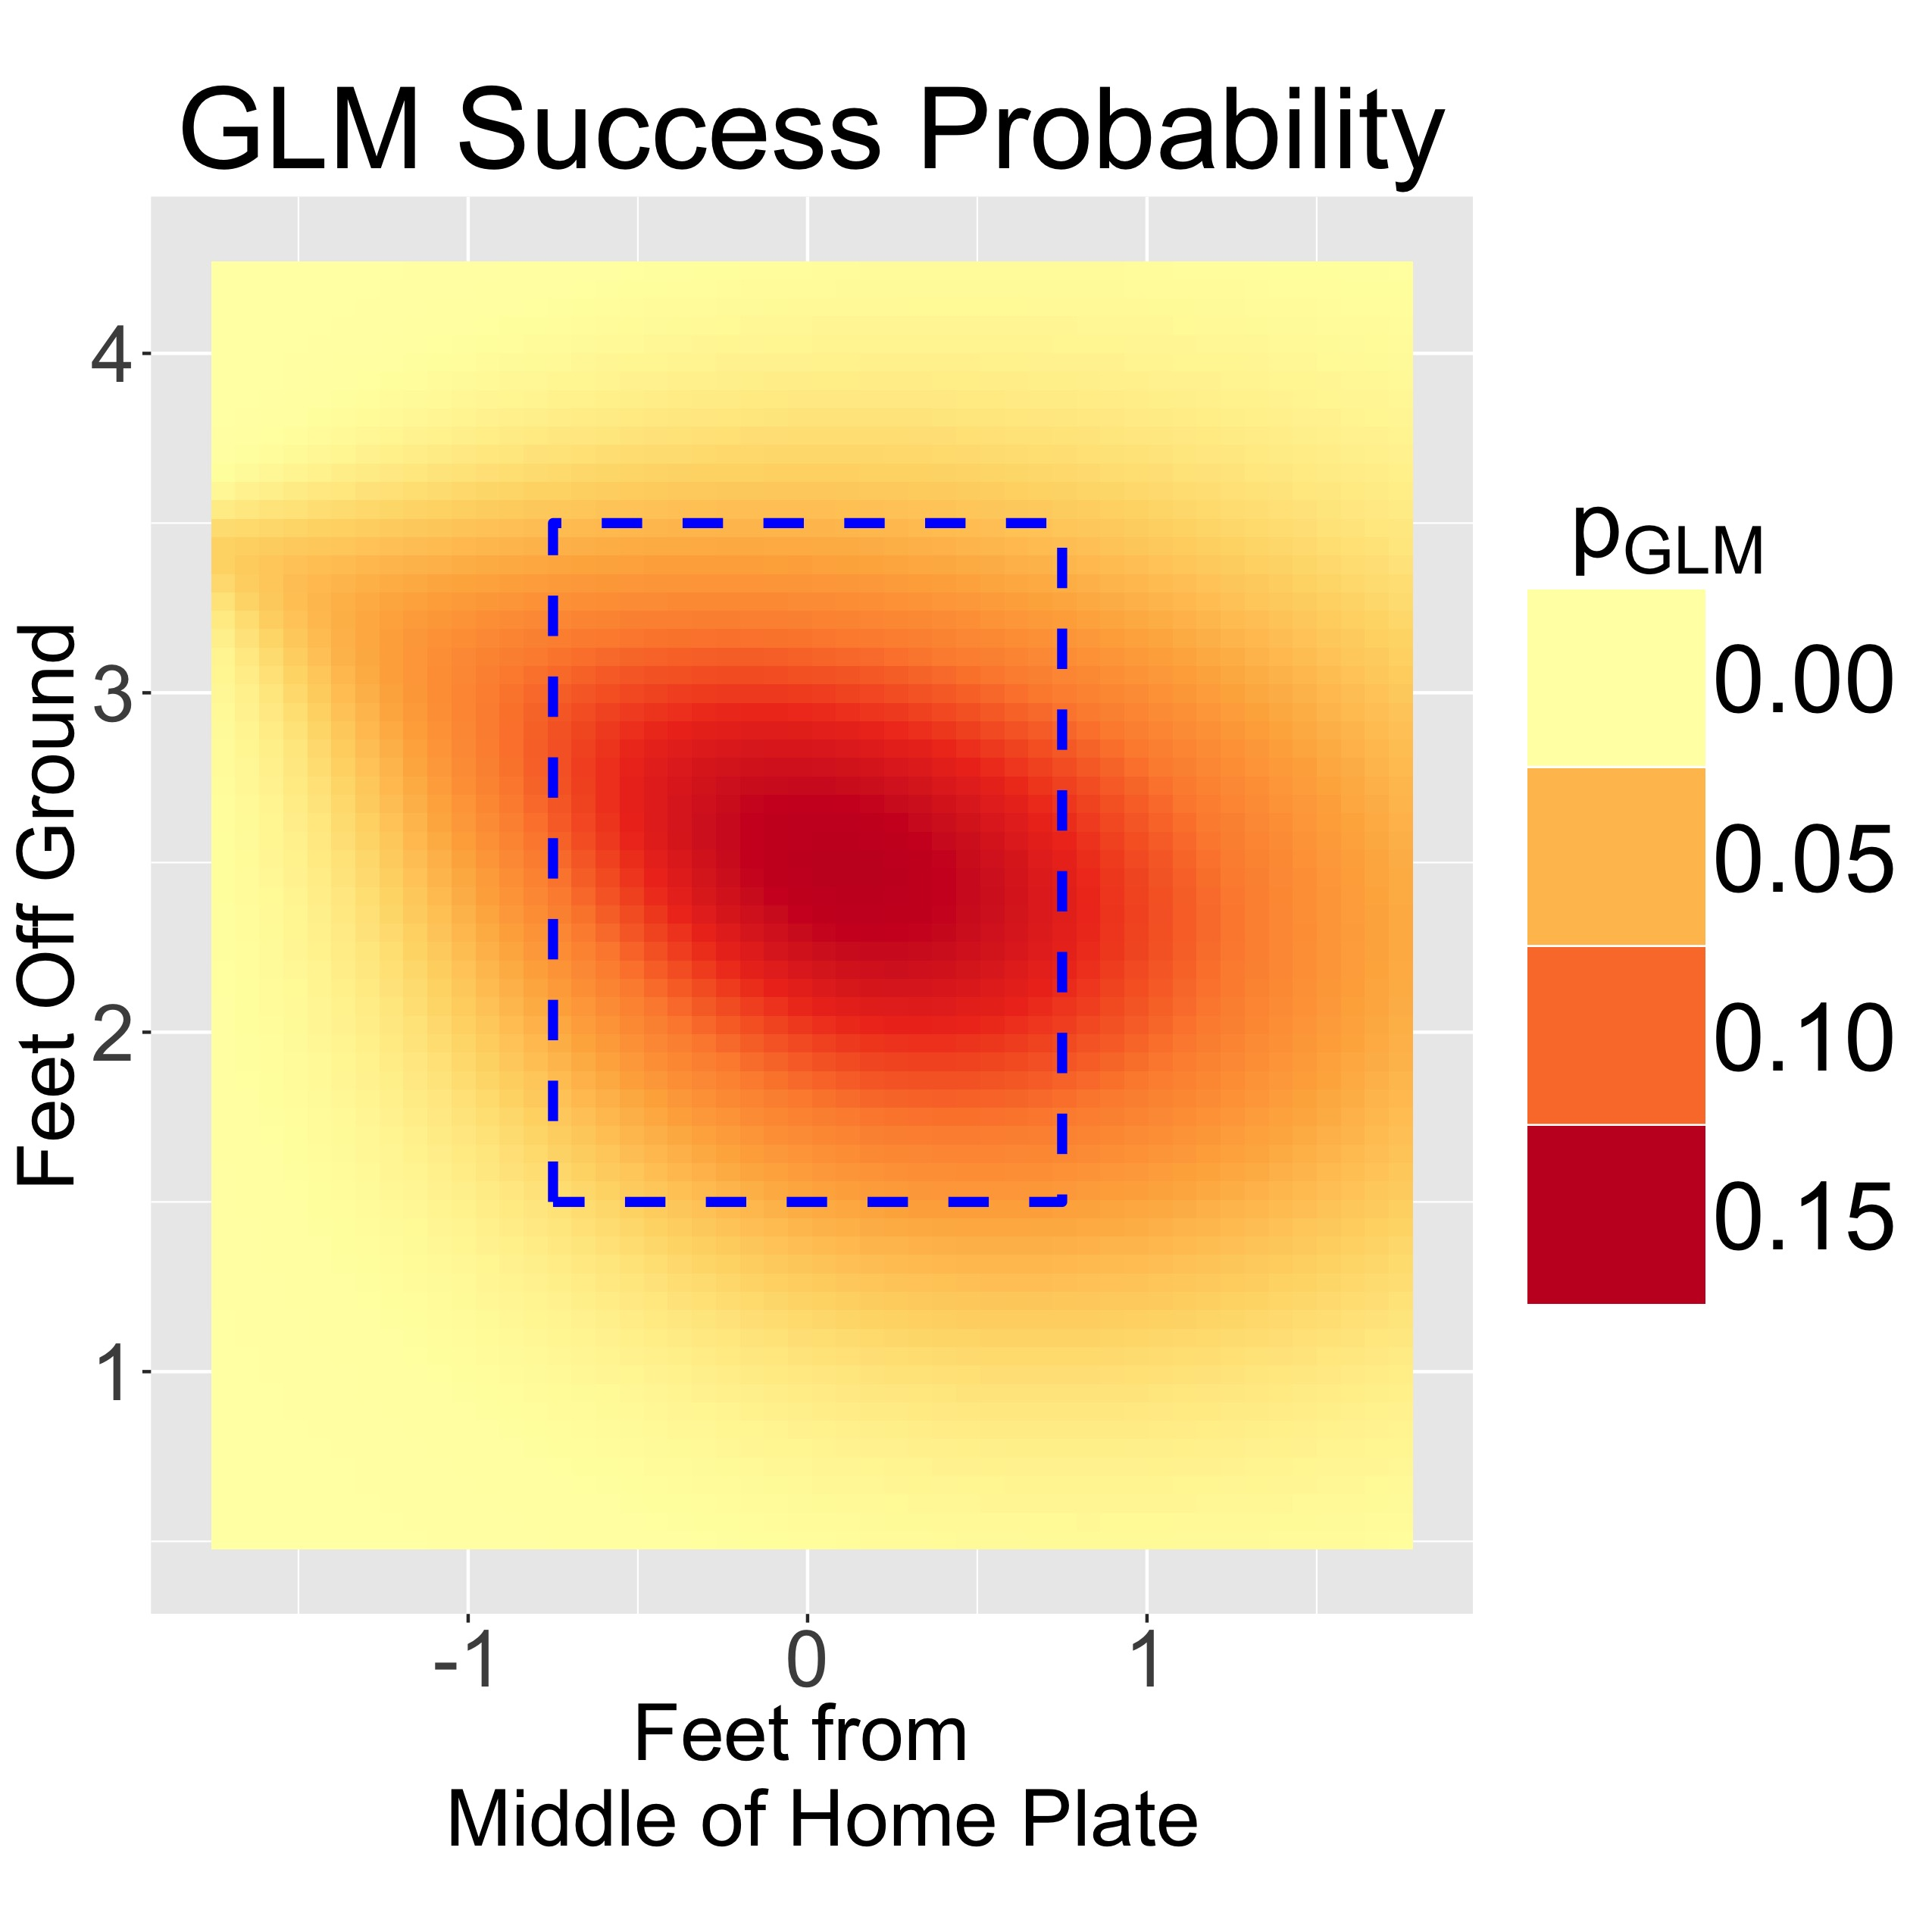
\includegraphics[scale=.08]{Images/Peralta_fit.jpg}
    \caption{Jhonny Peralta variable-resolution heat map and generalized linear model fit.}
  \end{figure}

\subsection{Hosmer-Lemeshow Goodness of Fit Test} % ================

The widely accepted Pearson $\chi^{2}$ test assesses goodness of fit for models fit with covariates that provide natural groupings. Continuous covariate models, however, need an imposed grouping mechanism. \cite{Hosmer2013} created a procedure with a grouping mechanism, and provided a goodness of fit test for logistic regression models with continuous covariates. 

Define Bernoulli outcome vector $\pmb{y}' = (y_{1}, y_{2}, \dots, y_{n})$, and logistic regression model fitted probability vector $\hat{\pmb{y}}' = (\hat{p}_{1}, \hat{p}_{2}, \dots, \hat{p}_{n})$, where $E(y_{i}) = p_{i}$. Then, arrange fitted values $\hat{p}_{1}, \hat{p}_{2}, \dots, \hat{p}_{n}$ in ascending order, and divide them into $g$ groups according evenly spaced percentiles: $1/g, 2/g, \dots g/g$. Therefore, $\text{Group 1} = \{\hat{p}_{i}|0 < \hat{p}_{i} < p_{1} \text{ where } \hat{\text{F}}(p_{1})=1/\text{g} \}$, with empirical CDF $\hat{\text{F}}(p)$. 

The Hosmer-Lemeshow goodness of fit statistic $\hat{C}$, equivalent to the Pearson $\chi^{2}$ statistic under this grouping structure, takes the following form.
$$ \widehat{C} = \sum_{k=1}^{g} \left[ \frac{(\text{o}_{1k}-\hat{e}_{1k})^{2}}{\hat{e}_{1k}} + \frac{(\text{o}_{0k}-\hat{e}_{0k})^{2}}{\hat{e}_{0k}}  \right] $$
where
$$ \text{o}_{1k} =  \sum_{j=1}^{n_{k}}y_{j},$$
$$ \text{o}_{0k} =  \sum_{j=1}^{n_{k}}(1-y_{j}),$$
$$ \hat{e}_{1k} = \sum_{j=1}^{n_{k}}\hat{p}_{j},$$
$$ \hat{e}_{0k} = \sum_{j=1}^{n_{k}}(1-\hat{p}_{j}),$$
and $n_{k}$ gives the number of observations in group k. $\widehat{C}$ simplifies to
$$ \widehat{C} = \sum_{k=1}^{g} \frac{(\text{o}_{1k}-n_{k}\bar{p}_{k})^{2}}{n_{k}\bar{p}_{k}(1-\bar{p}_{k})},$$
where $\bar{p}_{k}$ gives the group $k$ average predicted probability:
$$\bar{p}_{k} = \frac{1}{n_{k}}\sum_{j=1}^{n_{k}}\hat{p}_{j}$$

\cite{Hosmer1980} showed $\widehat{C}$ follows approximately a $\chi^{2}_{g-2}$, a chi-sq distribution with g-2 degrees of freedom, for simulated data. 

We performed the Hosmer-Lemeshow test, which has the standard goodness-of-fit null and alternative hypothesis.

\begin{align}
H_{0}: & \text{ Model well fit.} \\
H_{1}: & \text{ Model not well fit.}
\end{align}

We use g = 10, follwing the \cite{Hosmer2013} recommendation based on their simulations \cite{Hosmer1980}. Thus, the test statistic $\chi^{2} = 4.3758$, with eight degrees of freedom, gives a p-value of p = 0.8217. This encouraging result, a well fit model conclusion, lends credibility to the biomechanical covariate approach. Next, we consider heat map model confidence intervals.

\section{Heat Map Confidence Intervals}

A heat map presents, essentially, a two dimensional surface of point estimates. Each (x,y) point on the surface maps a point estimate of a parameter to a color. This effectively communicates the behavior of the parameter, or at least the point estimates, across the spatial domain. However, generally the usefulness of a point estimate depends on confidence interval accompaniment, and therein lies the challenge: how to present heat map confidence intervals (CIs)? This problem exists in numerous areas of application---any area where heat maps are used! ``I've heard this question asked in other areas,'' remarked Dr Sarah Emerson \citep{Emerson}. Indeed, Dr. Emerson reports that collaborative genomics research with Dr. Yanming Di lacked a satisfactory heat map confidence interval option \citep{Emerson}, (cite paper). In the next section we present the current heat map CI best practices, and examine how they can and should be improved.

\subsection{Current Best Practices}

The currect heat map confidence interval (CI) best practice simply presents two additional heat maps; the lower bound heat map and upper bound heat map. Sometimes the presentation includes maps for additional percentiles. For example, \cite{Cross2015} provides the following collection of heat maps to communicate prediction confidence.

  \begin{figure}[H]
	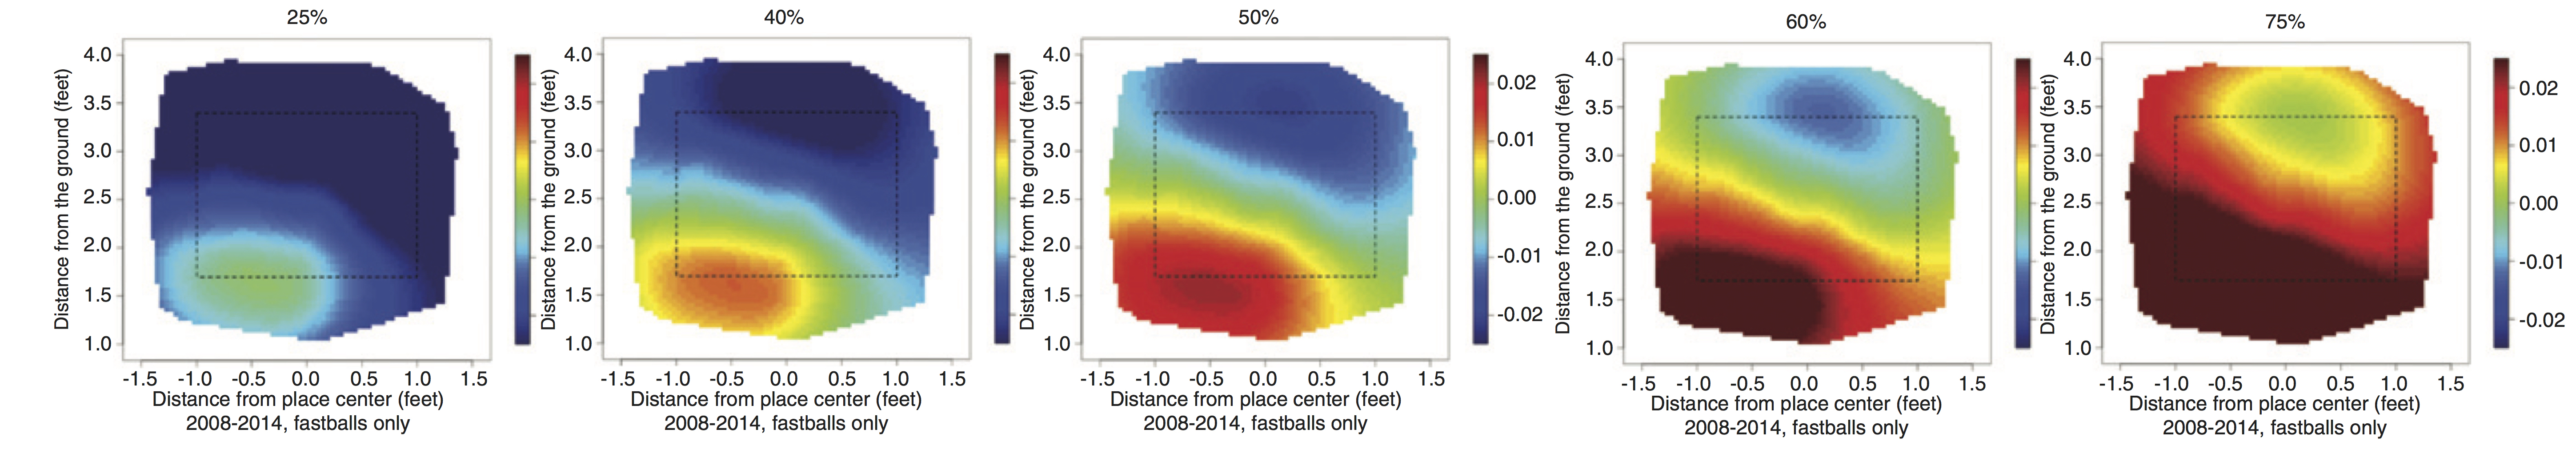
\includegraphics[scale=.07]{Images/CrossHMCI.jpg}
	\caption{In line with best practices, \cite{Cross2015} present four percentiles to convey confidence interval information for the point estimate heat map in the center. We submit this method resists easy comprehension and intuition.}
	\end{figure}

This heat map collection unfortunately confuses the audience with conceptually and intuitively inaccessible content. To elaborate, consider a hypothetical paremter and point estimate $\hat{\theta} = 2$, and hypothetical CI for $\hat{\theta}$ of (0,4). This combination makes plain its information content and structure; our familiarity with the number line contributes to easy comprehension.
  \begin{figure}[H]
  \centering
	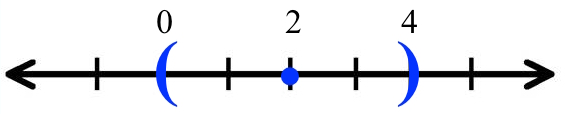
\includegraphics[scale=.6]{Images/NumberLine.jpg}
	\caption{Our brain readily understands and interprets the content of a confidence interval on the number line. On the other hand, our brain does not so easily understand and fill in intervals of the color spectrum.}
	\end{figure}
While one quickly, intuitively, and easily understands the content of the number line, we typically do not so easily fill in missing segments of the color spectrum. With heat map CIs, {\it colors} represent the point estimate and confidence bounds! A point estimate of ``green'' with a CI of (purple, red) confounds.
  \begin{figure}[H]
  \centering
	
\includegraphics[scale=.75]{Images/Lower.jpeg}
	
\includegraphics[scale=.75]{Images/SpectrumPE.jpg}
	
\includegraphics[scale=.75]{Images/Upper.jpeg}
	\caption{This representation of a confidence interval on the color spectrum demonstrates the interpretive challenge. What stream of colors exist between each bound and the point estimate?}
	\end{figure}

However, comprehension comes more easily with the entire spectrum within the confidence interval visible, as in Figure 6.
  \begin{figure}[H]
  \centering
	
\includegraphics[scale=.65]{Images/SpectrumCI.jpg}
	\caption{Interpretation of a colored confidence interval simplifies with the portions of the color spectrum between each bound and the point estimate visible. How do we achieve this for a heat map surface? This representation of a confidence interval on the color spectrum hints at the interpretive solution. }
	\end{figure}
This simplifies interpretation immensely. However, the problem remains; how do we acheive this for a heat map surface? A continuous model maps innumerable point estimates to a color on a surface, making a visible color spectrum CI for each point estimate infeasible. We propose a dynamic solution using RStudio's Shiny \citep{Shiny}, \citep{RStudio}.

\subsection{Shiny Innovation}

The inimitable RStudio created the Shiny framework to facilitate interactive web application development. Deployed directly out of the RStudio integrated development environment (IDE) \citep{IDE}, Shiny applications provide statisticians, all scientists in fact, with a powerful new tool for presenting analytical results. We take advantage of Shiny's capability to innovate a solution to the heat map CI problem articulated in the previous section.

Recall the GLM model heat map for Jhony Peralta. Figure 7 shows the lower and upper 95\% pointwise CI heat maps.

  \begin{figure}[H]
	\centering
	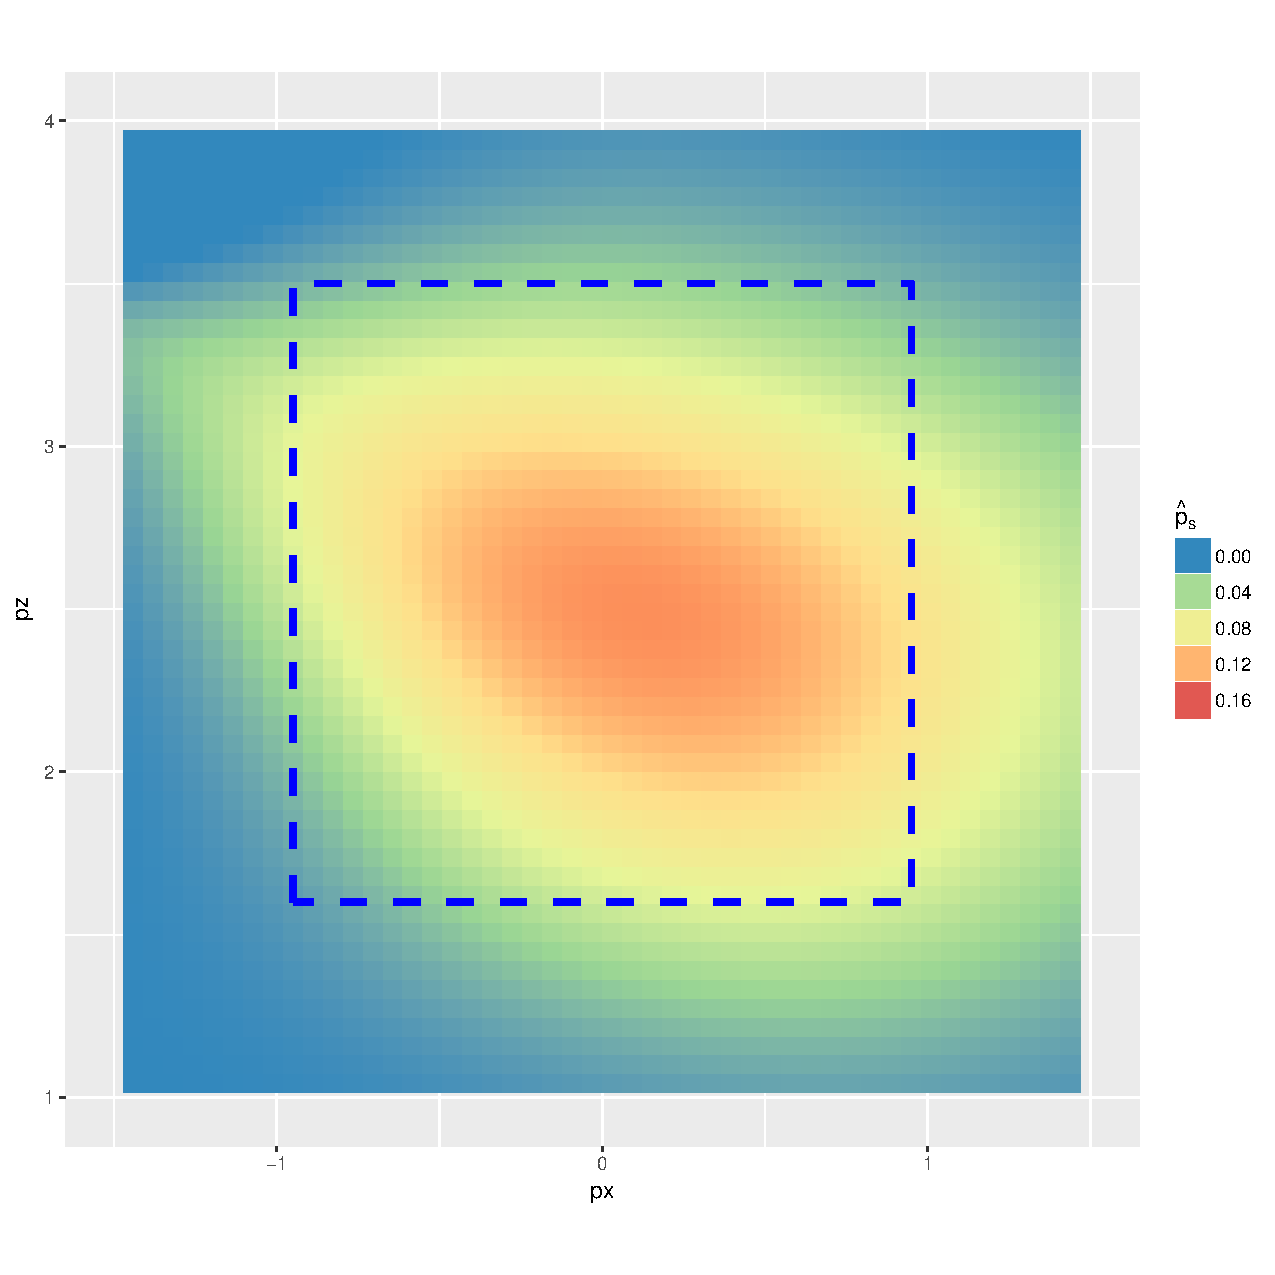
\includegraphics[scale=.25]{Images/Lower.pdf}
	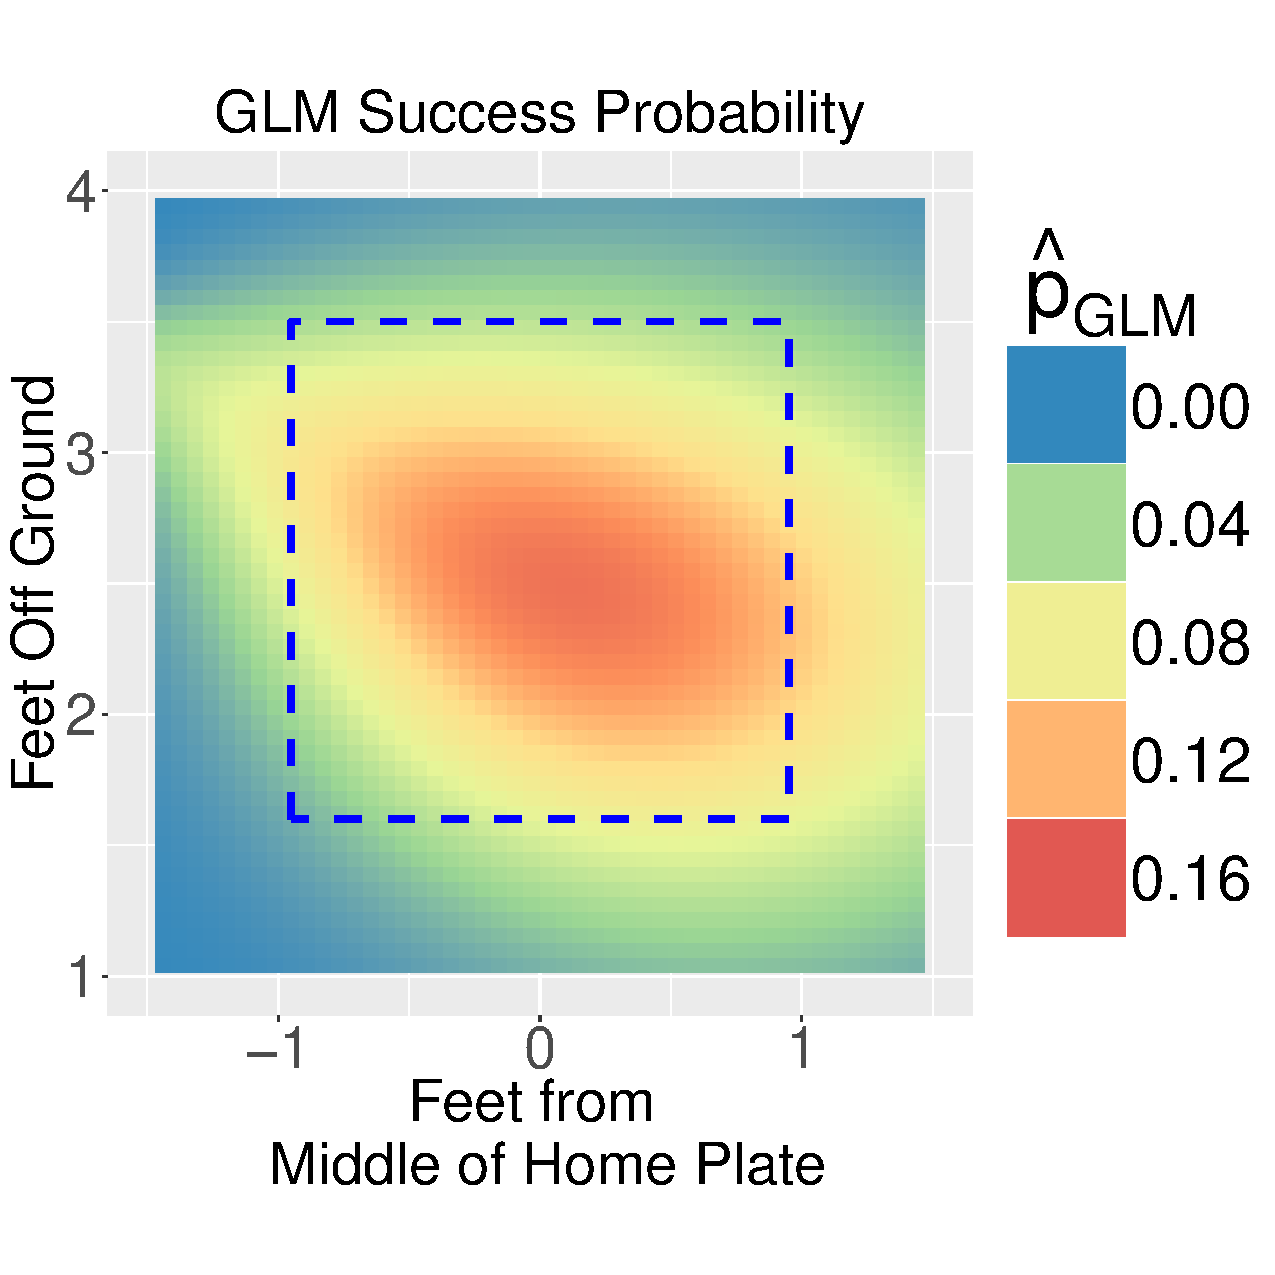
\includegraphics[scale=.25]{Images/Perralta_fit.pdf}
	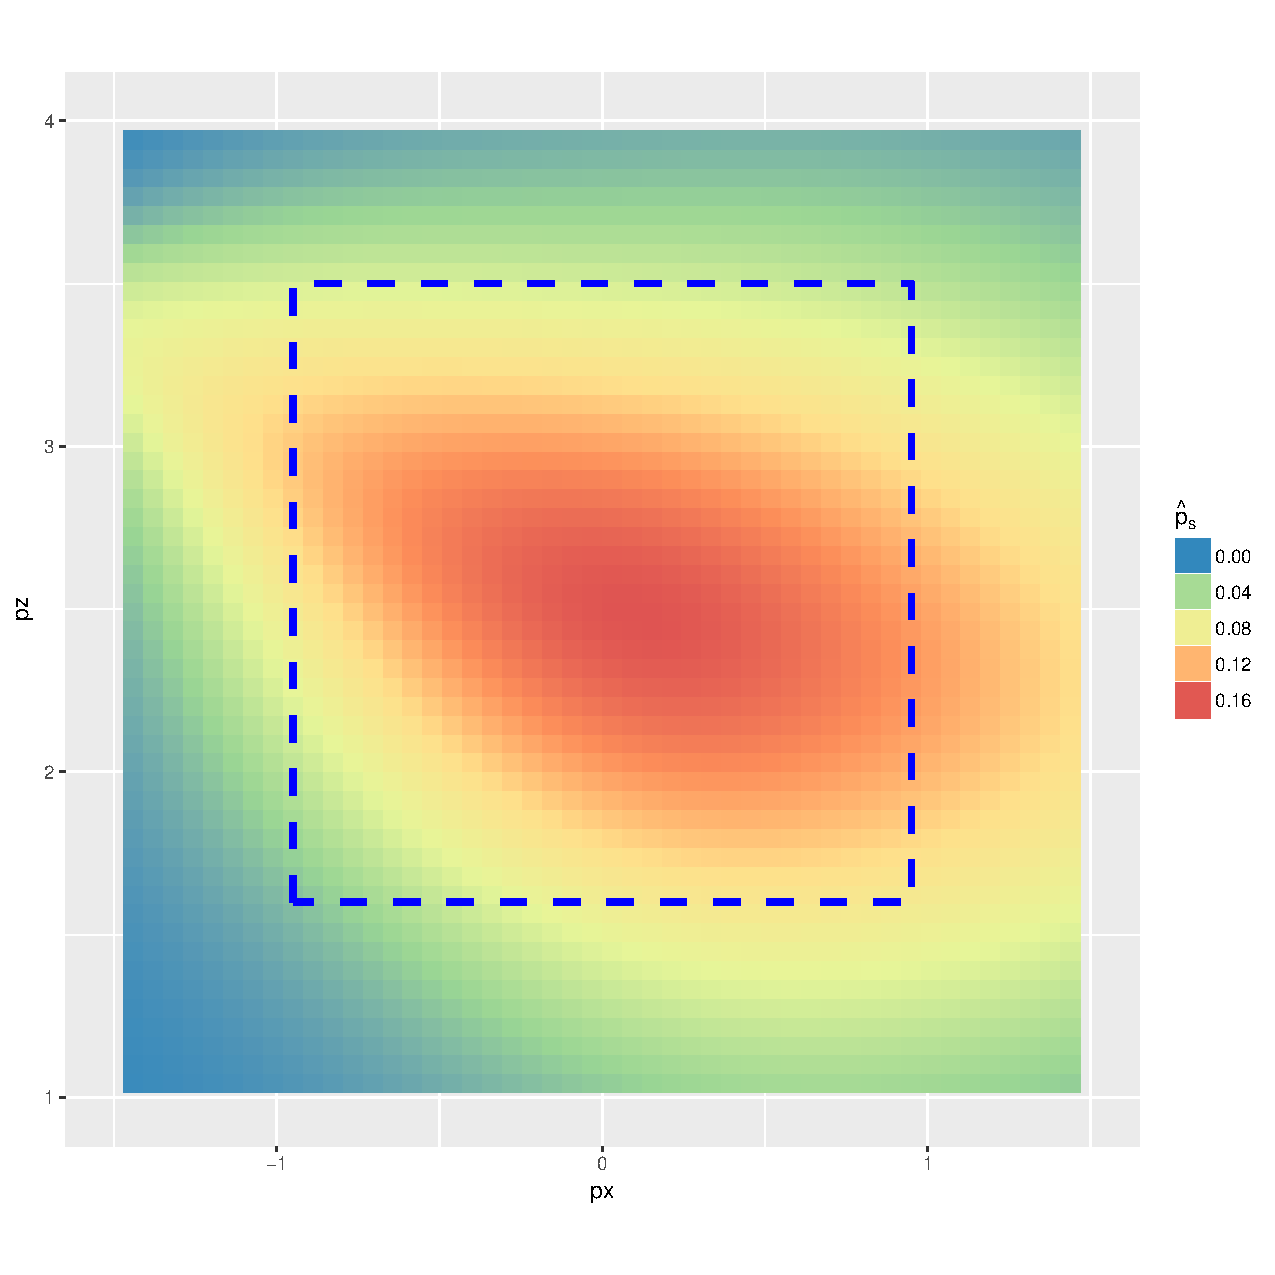
\includegraphics[scale=.25]{Images/Upper.pdf}
	\caption{Current best practices for a heat map confidence interval (CI). The generalized linear model fit for Jhony Peralta in the center, the pointwise CI lower bound on the left, and the pointwise CI upper bound on the right. Our interactive, dynamic heat map CIs will improve interpretability.}
	\end{figure}
The heat map on the left gives the lower bound of the 95\% CI, the heat map in the middle gives the model fit point estimates, and the heat map on the right gives the upper bound of the 95\% CI. We removed labels from the left and right heat maps for simplicity. The challenge lies in filling the space between the bounds and point estimate.

The static image of the interactive Shiny app in Figure 8 includes a slider in the lower left. The user adjusts the slider, a type of ``widget'' in Shiny, to move {\bf through} the CI.

  \begin{figure}[H]
	\centering
	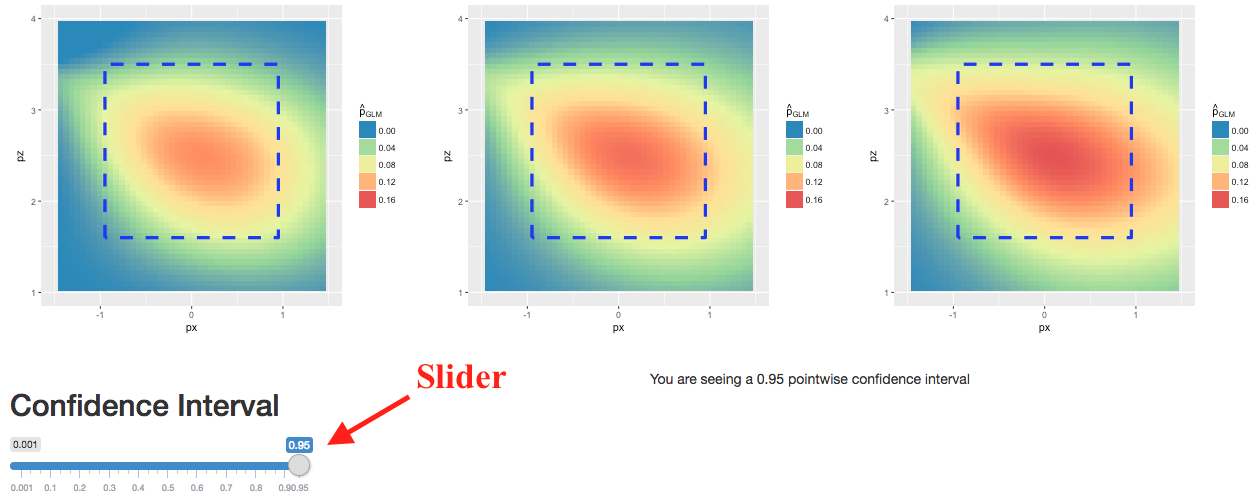
\includegraphics[scale=.35]{Images/95.png}
	\caption{We created interactive confidence intervals (CIs) with Shiny. The slider in the lower left allows the user to move {\it through} the CI. As the user adjusts the slider, the heat maps bounds adjust.}
	\end{figure}

As the user narrows the CI slider setting, the lower bound on the left and the upper bound on the right will look more and more similar to the point estimate heat map in the middle.

Figure 9 shows a sequence of static images in which the slider progressively narrows the CI.
  \begin{figure}[H]
	\centering
	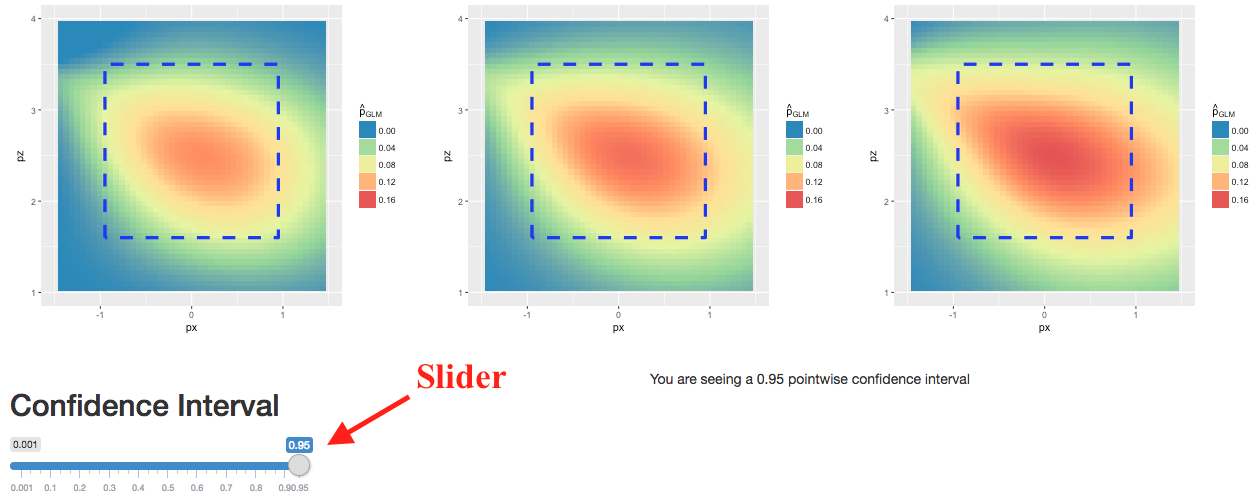
\includegraphics[scale=.25]{Images/95.png}
	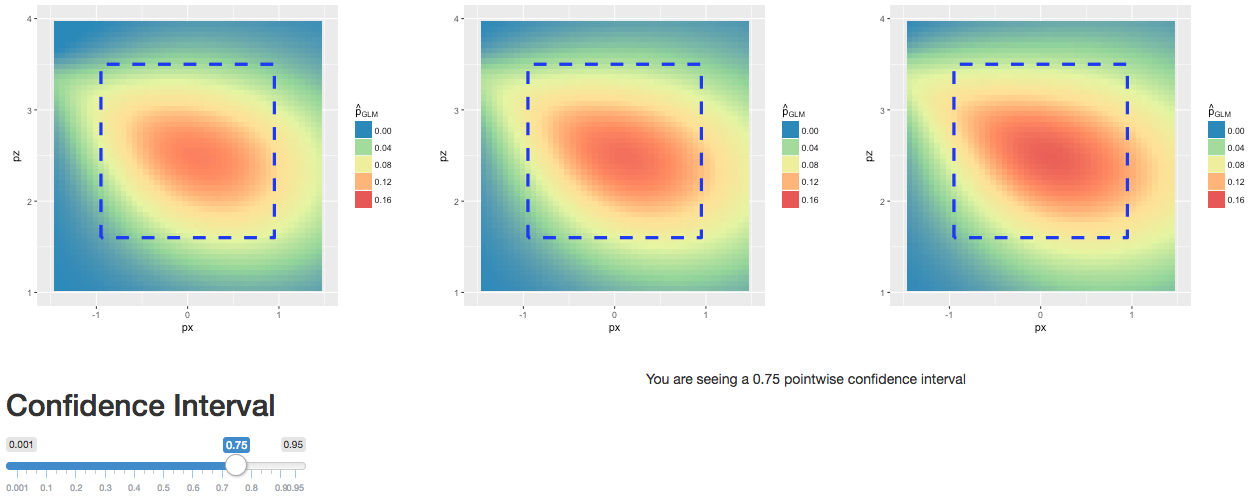
\includegraphics[scale=.25]{Images/75.png}
	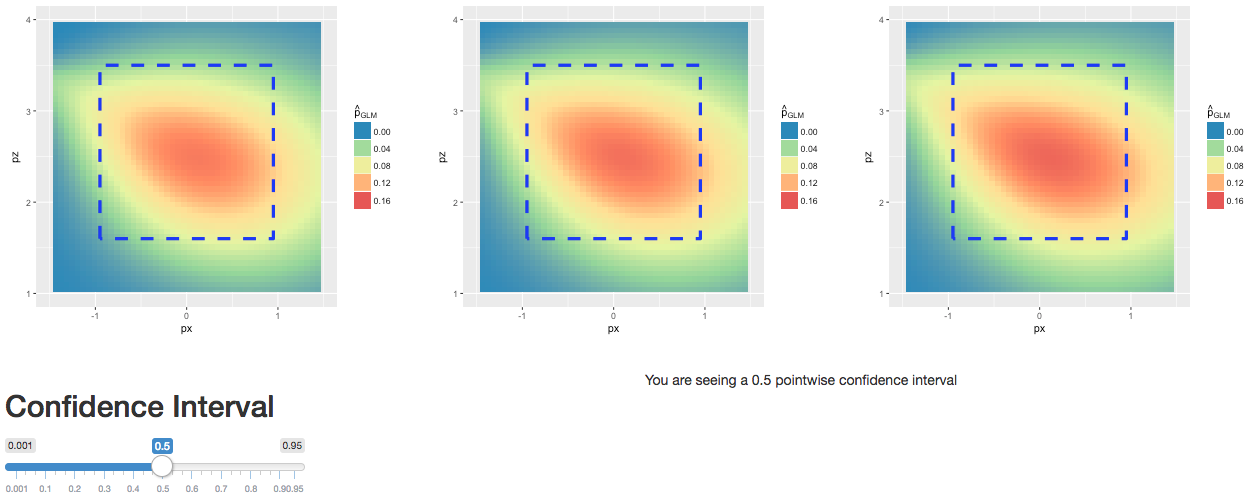
\includegraphics[scale=.25]{Images/50.png}
	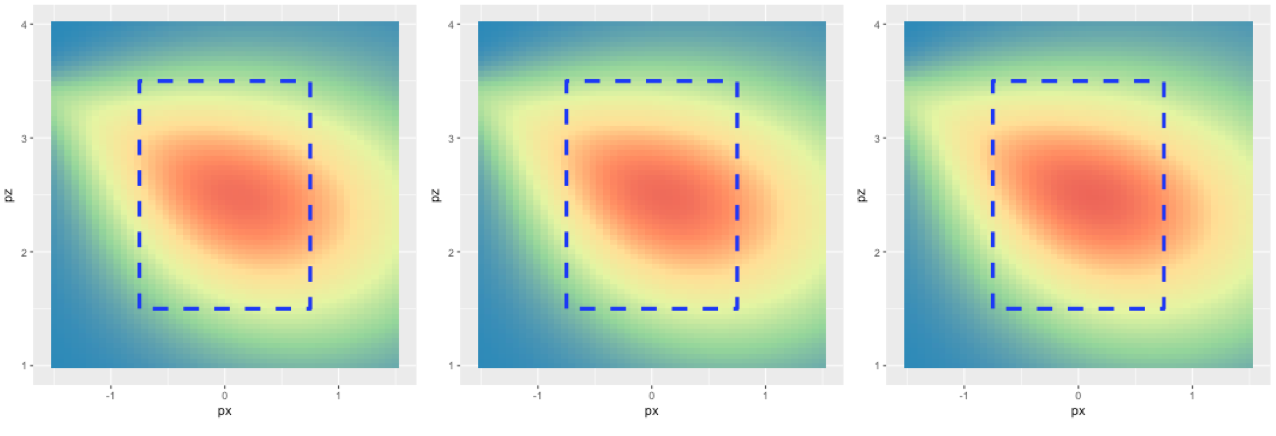
\includegraphics[scale=.25]{Images/25.png}
	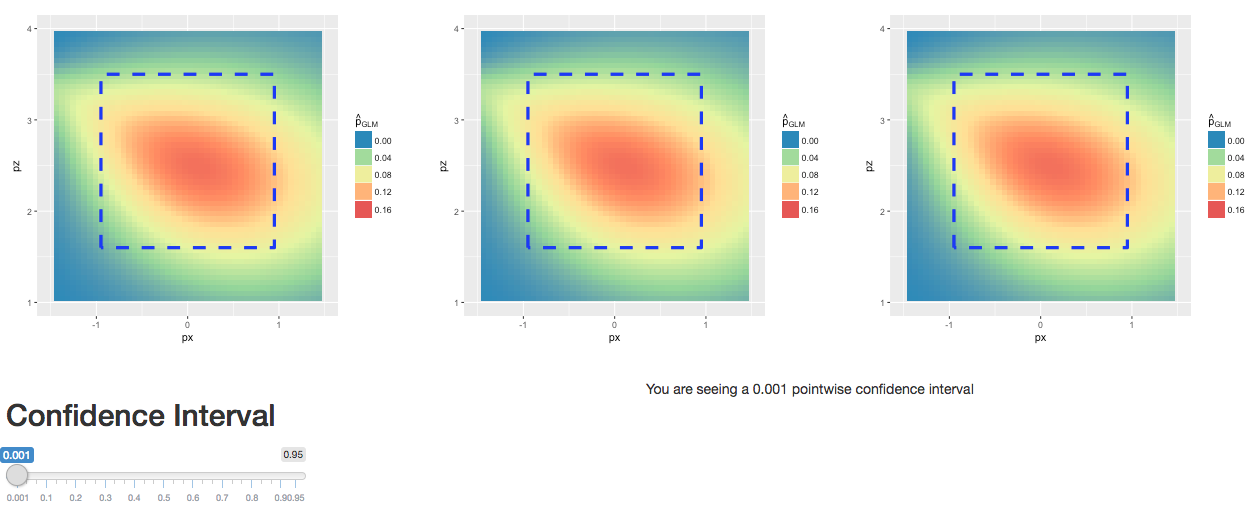
\includegraphics[scale=.25]{Images/0.png}
	\caption{A dynamic, Shiny, interactive heat map confidence interval. As the user adjusts the Shiny widget slider, the heat maps bounds adjust. This interactive app lets you move {\bf through} a heat map confidence interval.}
	\end{figure}

The slider for a row of three heat maps sits below that row. Moving from the top row to the bottom row, notice how the left and right-hand images increasingly resemble the middle image, until they all three match. While the paper version resembles that from \cite{Cross2015}, this interactive CI figuratively jumps off the page and comes to life as an interactive web application... and shines.

\section{Chapter Appendix}

\begin{tabular}[b]{ l | c | c | c | r }
    \hline
    Covariate         & $\beta_{i}$ & MLE   & SE     &      p  \\ \hline \hline
    N/A               & $\beta_{0}$ & -4.08 & 0.70 & $ <0.001$ \\ \hline
    r                 & $\beta_{1}$ &  1.19 & 0.51 & $  0.018$ \\ \hline
    $\theta$          & $\beta_{2}$ & -1.93 & 1.90 & $  0.311$ \\ \hline
    $r*\theta$        & $\beta_{3}$ & -1.64 & 0.70 & $  0.064$ \\ \hline
    $r^{2}$           & $\beta_{4}$ & -0.32 & 0.09 & $ <0.001$ \\ \hline
    $\theta^{2}$      & $\beta_{5}$ & -3.92 & 1.10 & $ <0.001$ \\ \hline
    $r^{2}*\theta^{2}$& $\beta_{6}$ & -0.46 & 0.21 & $  0.025$ \\ \hline
    \hline
\end{tabular}
